\documentclass[a4paper,UKenglish,cleveref, autoref, thm-restate]{lipics-v2021}

\usepackage[utf8]{inputenc}
\usepackage[T1]{fontenc}

\usepackage{amsmath, amssymb, amsthm, mathtools}
\usepackage{dsfont}
\usepackage{mathrsfs}
\usepackage{thmtools}
\usepackage{stmaryrd}

\usepackage{tikz}
\usetikzlibrary{arrows.meta,automata,positioning,calc,trees}
\usepackage{tikz-cd}
\usepackage{graphicx}

\usepackage{caption}

\usepackage{hyperref}

\usepackage{color}
\usepackage{xcolor}


\usepackage[hyperref,electronic]{knowledge}
\knowledgeconfigure{label scope=false, notion, quotation, protect quotation={tikzcd, automata}}

\input{macros}
\input{tree-uniformisation.kl}


\title{Decidability of MSO Uniformisation on Finite Trees}

\author{Thomas Colcombet}
	{CNRS, IRIF, Universit\'e Paris Diderot, France}
	{thomas.colcombet@irif.fr}
	{https://orcid.org/0000-0001-6529-6963}
	{}

\author{Yago Iglesias Vázquez}{Universit\'e Paris Diderot, France}{me@yagoiglesias.fr}{}{}
\nolinenumbers


\authorrunning{T. Colcombet, Y. Iglesias Vázquez} 

\Copyright{Thomas Colcombet, Yago Iglesias Vázquez} 

\ccsdesc[500]{Theory of computation~Finite Model Theory}
\ccsdesc[500]{Theory of computation~Algebraic language theory}
\ccsdesc[500]{Theory of computation~Regular languages}

\keywords{MSO, uniformisation, finite state automata, trees} 

\category{} 

\relatedversion{} 

\begin{document}

\maketitle

\begin{abstract}
	We study "uniformisation" for "MSO formulas" over "unordered finite binary trees". A "formula" $\psi(X)$ "uniformises" $\phi(X)$
	if it selects at most one witness $X$ and, whenever $\phi(X)$ has a witness, $\psi(X)$ picks one. We show that,
	using symmetry-preserving automata ("order-insensitive automata"), it is decidable whether a
	given $\phi(X)$ admits such a "uniformiser", and in the positive case, we effectively construct $\psi(X)$. Our procedure constructs from $\phi(X)$
	an "order-insensitive" "deterministic bottom-up tree automaton", checks whether that "automaton@DBUA" "accepts" every "tree", and, when
	it does, extracts from its "transition relation" an "MSO-formula" that uniformly selects a witness. This reduces "MSO uniformisation"
	on "finite trees" to a simple "automata universality" test and a "formula" extraction step.
\end{abstract}

\section{Introduction}

"Monadic second‐order logic" ("MSO" for short) is a well-studied fragment of second-order logic with wide-ranging applications in graph theory, automata theory, and formal verification.
In particular, its deep connection with automata theory has been extensively explored. It is well known that MSO over finite words is equivalent in expressive power to
finite-state automata~\cite{Buchi60}.

This correspondence extends beyond words: automata can also be defined to run on "trees". Over "finite trees", "MSO logic" remains equivalent in expressive power to finite-state
tree automata~\cite{TW68, Don70}. This connection enables the use of automata-theoretic techniques to reason about "trees", one of the most fundamental and widely studied data
structures.

A classical challenge in this context is the "uniformisation problem": given an "MSO-formula" $\phi(X)$ that asserts the existence of a set $X$ satisfying a certain property,
is it possible to define another "MSO-formula" $\psi(Y)$ that selects \emph{at most one} such set for each "tree", in a way that agrees with $\phi(X)$ whenever it is satisfiable? We
formalize this notion in \Cref{sec:uniformisation}, \Cref{def:uniformiser}.

This problem has been studied in various settings. A comprehensive survey is provided in~\cite{Cara15}. Positive results are known for finite words~\cite{Choffrut1999},
and infinite words, where every MSO-definable relation admits an MSO-definable uniformising function~\cite{Siefkes1975, Choffrut1999, Rabin07}. In contrast, uniformisation
is not possible in general for infinite binary trees~\cite{GS83}.
In this work, we study "MSO uniformisation" over a different class of structures: \emph{finite, unordered, labeled binary trees}.
All of the technical work is performed using only automata that preserve structural symmetry,
\ie they are unable to distinguish between left and right "subtrees".

The central question addressed in this paper is:

\begin{problem}[""uniformisation"" problem]\label{prob:uniformisation-problem}
\AP Given an "MSO-formula" $\phi(X)$, does there exist a "uniformiser" $\psi(X)$?
\end{problem}

Our main result, \Cref{theorem:main}, is that this question is \emph{decidable}, and in the positive case, a "uniformiser" $\psi(X)$ can be effectively constructed. Concretely, we translate $\phi(X)$ into a
"deterministic bottom-up tree automaton" whose "transition map" is "order-insensitive" -- closed under sibling swaps. We then perform a "universality" check on this
automaton -- does it accept every "tree"? -- and, when it does, we extract from its transitions an "MSO-formula" that uniformly selects a witness.

This paper makes two main contributions:
\begin{itemize}
	\item It demonstrates the equivalence between "MSO uniformisation", "definability", and "automorphism" invariance, \Cref{lem:main-result},
	\item It extends the decidability of "MSO uniformisation" to "finite binary trees", \Cref{theorem:main}.
\end{itemize}


\paragraph*{Structure of the paper.} The remainder of the paper is structured as follows:
\Cref{sec:definitions} introduces the necessary definitions, notations and classical results on "trees", "automata@DBUA", and "MSO logic", with an emphasis on the "order-insensitive"
variant of tree automata.
In \Cref{sec:uniformisation}, we define "uniformisation" and present our main result, proving that the "uniformisation problem" is decidable for "unordered finite binary trees".

In this paper notions are hyperlinked to their definitions, reading the paper in electronic form is recommended.

\section{Definitions} \label{sec:definitions}

In this section, we review classical concepts related to "trees", "automata@DBUA", and "logic@MSO".
\Cref{sec:trees} establishes our notation for "trees".
\Cref{sec:automata} provides a brief overview of "bottom-up tree automata@DBUA".
\Cref{sec:OrderAutomata} introduces an "order-insensitive" variant of these automata, and
\Cref{sec:UniversalityAutomata} defines a corresponding "universality" test.
Finally, \Cref{sec:MSO} describes how to translate between "MSO formulas" and "order-insensitive automata".
\subsection{Trees}\label{sec:trees}

This first subsection contains the definition of the "trees" we are working with. Other equivalent definitions of "trees" and
automata are possible~\cite{Thomas1997, tata}, but we have chosen this one because it is more intuitive, without adding much complexity to the proofs.

\begin{definition}
	\AP A ""tree"" over an alphabet $\Sigma$ is recursively defined as follows:
	\begin{itemize}
		\item $a$, where $a \in \Sigma$;
		\item $a(t,t')$, where $a \in \Sigma$ and $t, t'$ are "trees".
	\end{itemize}
	We call the ""root"" of a "tree" the first "node" in its definition.
	We denote the ""children"" of a "tree" $t$ as $t'$ and $t''$ in the case of $t = a(t',t'')$.
	The set of all "trees" over $\Sigma$ is denoted $\intro* \tree_{\Sigma}$.
	A subset of $\tree_{\Sigma}$ is called a ""tree language"" (or "language" for short).
\end{definition}

\begin{figure}[h]
	\centering

	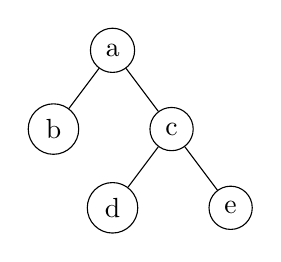
\begin{tikzpicture}[
			level distance=1cm,
			sibling distance=1.5cm,
			every node/.style = {draw, circle}
		]

		\node {a}
		child { node {b} }
		child { node {c}
				child { node {d} }
				child { node {e} }
			};

	\end{tikzpicture}

	\caption{Concrete "tree" corresponding to $a(b, c(d, e))$.}
\end{figure}

This recursive structure induces a natural notion of position within a "tree".

\begin{definition}
	\AP The set of ""nodes"" of a "tree" $t$, denoted $\Nodes t$, is defined as the set of binary strings (words over $\{0,1\}$)
	that represent paths from the "root" to each "node":
	\[
		\intro* \Nodes t =
		\begin{cases}
			\{\varepsilon\}                      & \text{if } t = a          \\
			\{\varepsilon\} \cup \setdef{0u}{u \in \Nodes {t'}}
			\cup \setdef{1u}{u \in \Nodes {t''}} & \text{if } t = a(t', t'')
		\end{cases}
	\]

	A "node" is thus the path from the "root" to a particular position in the "tree".
\end{definition}

\begin{example}
	Let $t := a(b, c(d, e))$. We compute:
	\[
		\Nodes b = \{\varepsilon\}, \quad \Nodes{c(d, e)} = \{\varepsilon, 0, 1\}
	\]
	\[
		\Nodes t = \{\varepsilon\} \cup \{0\} \cup \{1, 10, 11\} = \{\varepsilon, 0, 1, 10, 11\}
	\]
\end{example}


Among the "nodes", some are distinguished as "leaves", "nodes" without "children".
\begin{definition}
	\AP The ""leaves"" of a "tree" $t$ are defined as follows:
	\[
		\intro* \Leaves t = \begin{cases}
			\varepsilon                              & \text{if } t = a         \\
			\setdef {0u} {u \in \Leaves {t'}}
			\cup \setdef {1u} {u \in \Leaves {t''} } & \text{if } t = a(t',t'')
		\end{cases}
	\]

	\AP We can see that $\Leaves t \subseteq \Nodes t $ and we call ""internal nodes"" the set $\Nodes t \cap \Leaves t$
\end{definition}


Each "node" in a "tree" carries a symbol from the alphabet.
\AP Given a "tree" $t$ , we can access the ""label"" of a "node"
thanks to the function $\intro* \tlabel t {\cdot}$ :
\[
	\tlabel t n =   \begin{cases}
		a               & \text{if } t = a \text{ and } n = \varepsilon         \\
		a               & \text{if } t = a(t',t'') \text{ and } n = \varepsilon \\
		\tlabel {t'} m  & \text{if } t = a(t',t'') \text{ and } n = 0m          \\
		\tlabel {t''} m & \text{if } t = a(t',t'') \text{ and } n = 1m
	\end{cases}
\]

We often need to refer to the "subtree" rooted at a particular "node".
\AP We introduce the notation $\intro* \subtree t n$ to refer to the ""subtree""
of $t$ rooted at the "node" $n$. This can be computed as follows:
\[
	\subtree t n =   \begin{cases}
		t                & \text{if }  n = \varepsilon                  \\
		\subtree {t'} m  & \text{if } t = a(t',t'') \text{ and } n = 0m \\
		\subtree {t''} m & \text{if } t = a(t',t'') \text{ and } n = 1m
	\end{cases}
\]

The "ancestor relation" captures the natural hierarchical structure of a "tree": a "node" $x$ is an "ancestor"
of a "node" $y$ if $y$ is located in a "subtree" rooted at $x$.

\begin{definition}
	\AP Let $t$ be a "tree" and $x, y \in \Nodes t $. We define the ""ancestor"" relation as:
	\[
		x \intro* \ancestor y \tiff \exists z \in \Nodes t ,\, y = xz
	\]
\end{definition}

\begin{remark}
	Note that this order does not depend on the left or right position of the "children", \ie it preserves
	"order-insensitivity", this will be explored in the following sections.
\end{remark}


\subsection{Automata over trees}\label{sec:automata}

In this subsection we aim to define the basics of tree automata in a comprehensive way, adding as much detail as possible to the proofs. For reference,
one can look at more advanced books on this topic \cite{tata,bookautomata} and the survey \cite{Thomas1997}.

In classical automata theory, we analyze deterministic finite automaton (DFA), wich assign a unique state to each prefix of
a word, updating this state at each step using a transition function, ussualy reading the input from left to right.

A "deterministic bottom-up tree automaton" ("DBUA") generalizes this idea to "trees": instead of reading a linear word, it reads a
a "tree" where each "node" carries a symbol from a fixed alphabet. Rather than scanning from left to right, it proceeds
bottom-up, computing "states" at each "node" by combining the states of its "children" :
the automaton aggregates the information from those "subtrees" to assign a "state" to the parent.

The idea is to recursively assign a "state" to each "node" of the "tree":
\begin{itemize}
	\item At the "leaves", the "state" is determined directly from the symbol via a function $\init$, just as a DFA starts in a particular initial state.
	\item A DFA transitions based on the current letter and the state reached by the previous letters.
	      Similarly, when a "DBUA" reaches an "internal node", it transitions based on the "states" reached by its "children" and the "label" associated to the "node".
	\item Finally, the "state" assigned to the "root" tells us whether the whole "tree" is "accepted",
	      depending on whether it belongs to a set of "final states".
\end{itemize}

We now state the formal definitions.

\begin{definition}
	\AP A ""deterministic bottom-up tree automaton"" (\reintro*"DBUA") is a tuple $(\Sigma, Q, \init, \deltaA, F)$ where:
	\begin{itemize}
		\item $\Sigma$ is an alphabet.
		      \itemAP $Q$ is a finite set of ""states"".
		      \itemAP $\intro*\init : \Sigma \to Q$ is a function that initializes the ""initial states"" of the "leaves".
		      \itemAP $\intro*\deltaA : Q \times Q \times \Sigma \to Q$ is the ""transition map"".
		      \itemAP $F \subseteq Q$ is the set of ""final states"".
	\end{itemize}
    We often use $\init_a$ to denote $\init(a)$ for $a \in \Sigma$ and $\deltaA_a$ to denote $\deltaA(\cdot, \cdot, a)$ for $a \in \Sigma$.
\end{definition}

\begin{definition}
	\AP The ""interpretation"" of a "DBUA" $A = (\Sigma, Q, \init, \deltaA, F)$  over an alphabet $\Sigma$ is defined as follows:
	\begin{eqnarray*}
		\intro* \interpret A ~: \tree_{\Sigma} &\to& Q \\
		a &\mapsto& \init_a \\
		a(t,t') &\mapsto& \deltaA_a (\interpret A t, \interpret A {t'})
	\end{eqnarray*}

	We say that $A$ ""accepts"" a "tree" $t$ if $\interpret A t \in F$.

	We will sometimes use the notation $\deltaA(t)$ for the "interpretation" of $A$ over the "tree" $t$.
\end{definition}

\begin{example}[trees with at most two leaves]\label{ex:count-leaves}
	We define a "DBUA" $A = (\Sigma, Q, \init, \deltaA, F)$ that "accepts" exactly the "trees" with at most two "leaves". Let:
	\begin{itemize}
		\item $Q = \{0,1,2\}$, where $q=1$ means \textit{one leaf}, $q=2$ means \textit{two leaves},
		      and $q=3$ means \textit{more than two leaf}.
		\item $F = \{1,2\}$.
		\item For all $a \in \Sigma$, we define $\init_a = 1$.
		\item The "transition function" is defined by $\deltaA_a(q_1, q_2) = \min(q_1 + q_2, 3)$.
	\end{itemize}

	Intuitively, this automaton counts the number of "leaves" in the "tree", but caps the count at $3$ to detect when the number exceeds $2$.
	\Cref{fig:count-leaves} illustrates the execution of this automaton over a particular input.
\end{example}


\begin{figure}[h]
	\centering
	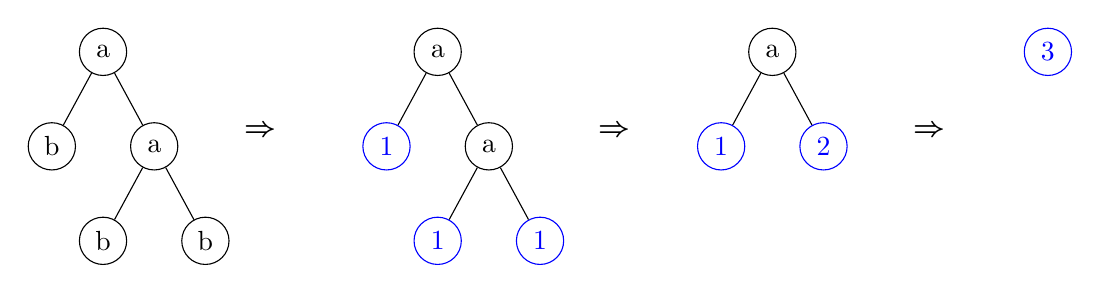
\begin{tikzpicture}[
			level distance=1.2cm,
			sibling distance=1.3cm,
			every node/.style={circle,draw,minimum size=6mm,inner sep=1pt},
			treenode/.style={circle,draw,minimum size=6mm,inner sep=1pt},
			scale=1, transform shape,
			state/.style={blue}
		]

		\node (t1) at (0,0) {a}
		child {node (t1b1) {b}}
		child {node (t1a2) {a}
				child {node (t1b3) {b}}
				child {node (t1b4) {b}}};

		\node at (2, -1) [draw=none] {$\boldsymbol{\Rightarrow}$};

		\node (t2) at (4.25,0) {a}
		child {node[state ](t2b1) {1}}
		child {node (t2a2) {a}
				child {node[state] (t2s2) {1}}
				child {node[state] (t2s3) {1}}};

		\node at (6.5, -1) [draw=none] {$\boldsymbol{\Rightarrow}$};

		\node (t3) at (8.5,0) {a}
		child {node[state] (t3s4) {1}}
		child {node[state] (t3a2) {2}};

		\node at (10.5, -1) [draw=none] {$\boldsymbol{\Rightarrow}$};

		\node[state] (t4) at (12,0) {3};

	\end{tikzpicture}
	\caption{Execution of the automaton of \Cref{ex:count-leaves} over the input $a(b,a(b,b))$}\label{fig:count-leaves}
\end{figure}


In the same way that we can define a non-deterministic automaton over strings, the same can be done for
tree automata using the same techniques. We will define them and give basic definitions on how to use them.

\begin{definition}
	\AP A ""non-deterministic bottom-up tree automaton"" (\reintro*"NBUA") is a tuple
	$(\Sigma, Q, \Init, \DeltaA, F)$ where:
	\begin{itemize}
		\item $\Sigma$ is an alphabet.
		\item $Q$ is a finite set of states.
		      \itemAP $\intro*\Init \subseteq \Sigma \times Q$ correspond to the possible states of the "leaves".
		      \itemAP $\intro*\DeltaA \subseteq Q \times Q \times \Sigma \times Q$ is the ""transition relation"".
		\item $F \subseteq Q$ is the set of "final states".
	\end{itemize}
\end{definition}

\begin{definition}
	\AP A ""run"" $\intro* \exec$ of an "NBUA" $A = (\Sigma, Q, \Init, \DeltaA, F)$ over a "tree" $t$ is :

	\begin{eqnarray*}
		\exec : \Nodes t  &\to& Q \\
		(\tlabel t b,  \exec (n) ) \in \Init &\text{ if }& n \in \Leaves t \\
		(\exec (n0), \exec (n1), \tlabel t n, \exec (n)) \in \DeltaA &\text{ if }& n \in \Nodes t \setminus \Leaves t
	\end{eqnarray*}

	We say that $\exec$ is an "accepting run" if $\exec (\varepsilon) \in F$ and $A$ "accepts" $t$ if
	$F \cap \setdef {\rho(\varepsilon)} {\text{$\rho$ "run" of~$A$ over~$t$}} \neq \emptyset$
\end{definition}


\begin{definition}
	\AP Let $A$ be an "NBUA". Its ""associated language"" is defined as:
	\[\intro* \lang A = \setdef {t \in \tree_{\Sigma}} {\text{exists $\rho$ a "accepting" "run" of $A$ over $t$}} \]
\end{definition}

\begin{remark}
	Just like in classical automata theory, we can see a "DBUA" $A = (\Sigma, Q, \init, \deltaA, F)$ as a special
	case of a "NBUA" $A' = (\Sigma, Q, \Init, \DeltaA, F)$ where:
	\begin{itemize}
		\item $\Init = \setdef{(a, \init_a)}{a \in \Sigma}$,
		\item $\DeltaA = \setdef{(q_1, q_2, a, \deltaA_a(q_1, q_2))}{q_1, q_2 \in Q, a \in \Sigma}$.
	\end{itemize}

	In this case, $A'$ has exactly one possible "run" on each "tree" :
	\begin{eqnarray*}
		\exec : \Nodes t  &\to & Q \\
		n  &\mapsto& \init_{\tlabel t n} \text{ if } n \in \Leaves t \\
		n  &\mapsto& \deltaA_{\tlabel t n}(\exec (n0), \exec (n1)) \text{ if } n \in \Nodes t  \setminus \Leaves t
	\end{eqnarray*}
\end{remark}


The following lemma shows the equivalence of both definitions.

\begin{lemma}
	Let $A$ be a "DBUA",
	\[ \lang A = \setdef {t \in \tree_{\Sigma}} {\interpret A t \in F} \]
\end{lemma}

\begin{proof}
	We will prove by induction on a "tree"~$t$ that (a) there exists a "run" of~$A$ over~$t$, and (b) for all "runs"~$\exec$ of $A$ over $t$, $\interpret A t = \exec (\varepsilon)$.
	We proceed by case distinction.
	\begin{itemize}
		\item If $t = a$. Let $\rho$ be defined by $\rho(\varepsilon)=\init_a$, then $\rho$ is a "run" of~$A$ over~$t$. We have proved (a).
		      Consider now some "run" $\rho$ of $A$ over~$t$. We have $\rho(\varepsilon)=\init_a=\interpret A a=\interpret A t$. We have proved  (b).

		\item If $t = a(t',t'')$. By induction hypothesis (a), there exists "runs"~$\rho'$ and $\rho''$ on~$t'$ and $t''$ respectively.
		      Let~$\rho$ be defined by $\rho(\varepsilon)=\deltaA_{t(\varepsilon)}(\rho'(\varepsilon),\rho''(\varepsilon))$,
		      $\rho(0u)=\rho'(u)$ for all $u\in\Nodes{t'}$ and $\rho(1u)=\rho''(u)$ for all~$u\in \Nodes{t''}$. Then $\rho$ is a "run" of~$A$ over $t$. We have proved (a).

		      Consider now some "run" $\rho$ of $A$ over $t$. Let~$\rho'(u)=\rho(0u)$ for all $u \in \Nodes {t'}$ and $\rho''(u)=\rho(0u)$ for all $u \in \Nodes {t''}$.
		      Then $\rho'$ is a "run" of~$A$ over $t'$ and $\rho''$ over $t''$. By induction hypothesis (b) twice, we know that $\rho'(\varepsilon)=\interpret A {t'}$ and $\rho''(\varepsilon)=\interpret A {t''}$.
		      We have now $\rho(\varepsilon) = \deltaA_{t(\varepsilon)}(\rho'(\varepsilon),\rho''(\varepsilon)) = \deltaA_{t(\varepsilon)}(\interpret A {t'},\interpret A {t''}) = \interpret A t$. We have proved (b).
	\end{itemize}
\end{proof}


We aim now to show that, like in the classical theory, both "non-deterministic automata" and "deterministic@DBUA" ones have the same expressiveness power.
Since "DBUA" is a particular case of "NBUA" it suffices to show that each "language" accepted by an "NBUA" can also be accepted by a "DBUA".

\begin{definition}
	\AP Let $A = \NBUA$ be an "NBUA", we define the ""power set automaton"" of $A$, noted $\intro* \Det A$, as
	$\Det A = (\Sigma, \parts Q, \init, \deltaA, F')$ where:

	\begin{itemize}
		\item $\begin{aligned}[t]
				      \init      : \Sigma & \to \parts Q                              \\
				      a                   & \mapsto \setdef{q \in Q}{(a,q) \in \Init}
			      \end{aligned} $

		\item $\begin{aligned}[t]
				      \deltaA               : \parts Q \times \parts Q \times \Sigma & \to \parts Q                                                      \\
				      (X, Y, a)                                                      & \mapsto \setdef{q \in Q}{(x,y,a,q) \in \DeltaA, x \in X, y \in Y}
			      \end{aligned}$

		\item $F' = \setdef{X \in \parts Q}{X \cap F \neq \emptyset}$
	\end{itemize}
\end{definition}

\begin{theorem}\label{thm:determinisation}
	For all $N = \NBUA$ an "NBUA", the "power set automaton" verifies that
	\[
		\interpret {\Det N} t = \setdef {\rho(\varepsilon)}{\text{$\rho$ "run" of~$N$ over~$t$}} \text{ and } \lang N = \lang {\Det N}
	\]
\end{theorem}

\begin{proof}
	We will first show that for all "trees" $t$,
	\[
		\interpret {\Det N} t = \setdef {\rho(\varepsilon)}{\text{$\rho$ "run" of~$N$ over~$t$}}\ .
	\]
	We will prove this property by induction over $t$. We proceed by case distinction.
	\begin{itemize}
		\item If $t = a$, then
		      \begin{eqnarray*}
			      \setdef {\rho(\varepsilon)}{\text{$\rho$ "run" of~$N$ over~$t$}} &=&  \setdef {q \in Q} {(a,q) \in \Init} \\
			      &=& \interpret {\Det N} t\ .
		      \end{eqnarray*}
		\item If $t = a(t_1,t_2)$, then
		      by the induction hypothesis we know that
		      $\interpret {\Det N} {t_i} = q_i$ if and only if there exists a "run" over $t_i$ ending at $q_i$, for $i \in \set {1,2}$.

		      \begin{eqnarray*}
			      &&q \in \interpret {\Det N} t \\
			      &\text{if and only if}& q \in \deltaA_a (\interpret {\Det N} {t_1}, \interpret {\Det N} {t_2}) \\
			      &\text{if and only if}& q \in \setdef {q \in  Q} {(x_1,x_2,a,q) \in \DeltaA, x_1 \in \interpret {\Det N} {t_1}, x_2 \in \interpret {\Det N} {t_2}} \\
			      &\text{if and only if}& \exists x_1,x_2, (x_1,x_2,a,q) \in \DeltaA, x_1 \in \interpret {\Det N} {t_1}, x_2 \in \interpret {\Det N} {t_2} \\
			      &\text{if and only if}& \text{there exists a "run" over }  t_i  \text { ending at } x_i \text { for  } i \in \set {1,2} \text{ and } (x_1,x_2,a,q) \in \DeltaA\\
			      &\text{if and only if}& q \in \setdef {\rho(\varepsilon)}{\text{$\rho$ "run" of~$N$ over~$t$}}
		      \end{eqnarray*}
	\end{itemize}
	Then $ \interpret {\Det N} t = \setdef {\rho(\varepsilon)}{\text{$\rho$ "run" of~$N$ over~$t$}}$.\\

	We must now show that $\Det N$ "accepts" $t$ if and only if $N$ "accepts" $t$.
	\begin{eqnarray*}
		N \text{ "accepts" } t &\tiff& F \cap \setdef {q \in Q} {(a,q) \in \Init} \neq \emptyset \\
		&\tiff&   F \cap  \interpret {\Det N} t \neq \emptyset \\
		&\tiff& \interpret {\Det N} t  \in F' \\
		&\tiff& {\Det N} \text{ "accepts" } t
	\end{eqnarray*}
	and so $\lang N = \lang {\Det N}$.
\end{proof}


\subsection{Order-insensitivity}\label{sec:OrderAutomata}

We will define a particular kind of tree automata: the ones that do not distinguish between left and right "children".
That means that the "state" reached from the two "children" is the same if we swap them. These automata are
interesting because they respect the symmetries of "trees", which will pay an important role in \Cref{sec:uniformisation}.
While our definition of "trees" is ordered, \ie we can syntactically distinguish between left and right "children" of a "node",
for the rest of the paper we will only consider automata that do not distinguish between left and right "children", which means that
we will be essentially working over unordered trees, since we will be ignoring the order of the "children" in the "trees", and all of our results
will be valid for unordered trees.


\begin{definition}
	\AP An "NBUA" of "transition relation"~$\DeltaA$ is ""order-insensitive"" if for all "transitions@@relation" $(p,q,a,r) \in \DeltaA$, then
	$(q,p,a,r) \in \DeltaA$.
\end{definition}

\begin{remark}\label{def:order-insensitive}
	For a "DBUA" of "transition map"~$\deltaA$, it is "order-insensitive" if and only if
	$\deltaA_a (p,q) = \deltaA_a (q,p)$ for all "states"~$p,q$ and letter~$a$.
\end{remark}


\begin{figure}[h]
	\centering
	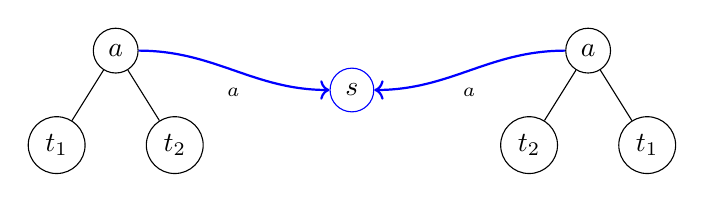
\begin{tikzpicture}[
			level distance=1.2cm,
			level 1/.style={sibling distance=1.5cm},
			every node/.style={draw, circle},
			baseline={(current bounding box.center)}
		]

		% Left Tree
		\node (root1) {$a$}
		child {node {$t_1$}}
		child {node {$t_2$}};

		% Right Tree
		\node (root2) at (6,0) {$a$}
		child {node {$t_2$}}
		child {node {$t_1$}};

		% State s
		\node[draw=blue] (s) at (3, -0.5) {$s$};

		% Arrows
		\draw[->, thick, draw=blue] (root1) to[out=0, in=180] node[draw=none, midway, below] {\(\deltaA_a\)} (s);
		\draw[->, thick, draw=blue] (root2) to[out=180, in=0] node[draw=none, midway, below] {\(\deltaA_a\)} (s);

	\end{tikzpicture}
	\caption{Illustration of "order-insensitivity" in a "DBUA" (see \Cref{def:order-insensitive}).
		Both "trees" yield the same state $s$ under the "transition map" $\deltaA_a$.}
	\label{fig:order-insensitivity}
\end{figure}



\begin{lemma}\label{lem:order-insensitive-det}
	If $N = \NBUA$ an "NBUA" is "order-insensitive", then $\Det N$ is also "order-insensitive".
\end{lemma}

\begin{proof}
	\begin{eqnarray*}
		\deltaA_a (X,Y) &=& \setdef {q \in Q} {(x,y,a,q) \in \DeltaA, x \in X, y \in Y} \\
		&=& \setdef {q \in Q} {(y,x,a,q) \in \DeltaA, x \in X, y \in Y}  \reason {$N$ is "order-insensitive"} \\
		&=& \deltaA_a (Y,X)
	\end{eqnarray*}
\end{proof}


Using both \Cref{thm:determinisation} and \Cref{lem:order-insensitive-det}, we can conclude that "order-insensitive" "NBUA" and "order-insensitive" "DBUA" are equivalent. We will
use them indiscriminately in the following sections, using the definition better suited to the context.

\subsection{Universality}\label{sec:UniversalityAutomata}

In this section, we define the "reachability set" of a "DBUA" and show that it can be used to decide "universality", which is the property of "accepting" every "tree".

\begin{definition}[""reachability set""]
	\AP Let $A = \DBUA$ a "DBUA", and let $\intro* \Reach A \subseteq Q$ be the smallest set such that:
	\begin{enumerate}
		\item $\init(a) \in \Reach A$ for all $a \in \Sigma$,
		\item $\deltaA(p, q, a) \in \Reach A$ for all $p, q \in \Reach A$ and $a \in \Sigma$.
	\end{enumerate}
\end{definition}

This set captures all "states" that can be reached by the automaton starting from the "leaves" and combining them using the "transition map".
In particular, it represents the set of all "states" that can be reached when the automaton processes all possible "trees", motivating the following lemma.

\begin{lemma}
	Let $A$ be a "DBUA", then:
	\[
		\Reach A = \setdef {\interpret A t} {t \in \tree_\Sigma}.
	\]
\end{lemma}

\begin{proofI}
	We prove the equality by showing both inclusions.
	\begin{itemize}
		\item For the direction $\Reach A \subseteq \setdef {\interpret A t} {t \in \tree_\Sigma}$, we proceed by induction over the construction of elements in $\Reach A$:
		      \begin{itemize}
			      \item If $r = \init(a)$ for some $a \in \Sigma$, then the "tree" $a$ satisfies $\interpret A a = \init(a) = r$.
			      \item If $r = \deltaA(p, q, a)$ where $p, q \in \Reach A$, then by the induction hypothesis there exist
			            $t', t'' \in \tree_\Sigma$ such that $\interpret A {t'} = p$ and $\interpret A {t''} = q$. Then the "tree" $t = a(t', t'')$ satisfies $\interpret A t = r$.
		      \end{itemize}

		\item For the direction $\setdef {\interpret A t} {t \in \tree_\Sigma} \subseteq \Reach A$, we use structural induction on a "tree" $t$:
		      \begin{itemize}
			      \item If $t = a$, then $\interpret A a = \init(a) \in \Reach A$.
			      \item If $t = a(t', t'')$, then by the induction hypothesis $\interpret A {t'}, \interpret A {t''} \in \Reach A$, so
			            $\interpret A t = \deltaA(\interpret A {t'}, \interpret A {t''}, a) \in \Reach A$.
		      \end{itemize}
	\end{itemize}
\end{proofI}

\begin{definition}
	\AP Let $A$ be a "NBUA". We say that $A$ is ""universal"" if it "accepts" every "tree".
\end{definition}

We can use the "reachability set" to decide whether an automaton is "universal". Intuitively, a "DBUA" is "universal" if
the only "states" it can reach are "final states". This is formalized in the following theorem.

\begin{theorem}\label{thm:universal-Reach}
	A "DBUA" $A = \DBUA$ is "universal" if and only if $\Reach A \subseteq F$.
\end{theorem}

\begin{proofI}
	\begin{itemize}
		\item Suppose $A$ is "universal". Then for all $t \in \tree_\Sigma$, we have $\interpret A t \in F$ because $A$ "accepts" $t$.
		      Since $\Reach A = \setdef {\interpret A t} {t \in \tree_\Sigma}$, we conclude that $\Reach A \subseteq F$.

		\item Conversely, suppose $\Reach A \subseteq F$. For any "tree" $t \in \tree_\Sigma$, we have $\interpret A t \in \Reach A \subseteq F$.
		      Hence, $A$ "accepts" $t$ and is therefore "universal".
	\end{itemize}
\end{proofI}

\begin{coro}\label{coro:univeral-Reach}
	A saturation algorithm based on $\Reach A$ decides "universality".
\end{coro}

\begin{proof}
	We can compute $\Reach A$ using a saturation algorithm that starts with the "initial states" and iteratively adds "states" reachable by the "transition map" until no new "states" can be added.
	Once we have computed $\Reach A$, we can check if it is a subset of the "final states". This algorithm will terminate because the number of "states" is finite,
	and it will decide "universality" by \Cref{thm:universal-Reach}.
\end{proof}

This algorithm will be used later in \Cref{sec:uniformisation} to decide "uniformisation".

\subsection{Monadic second-order logic on trees}\label{sec:MSO}
In this subsection, we introduce "monadic second-order logic" ("MSO") over "finite binary trees", and examine its relationship with
"non-deterministic bottom-up automata", in particular with "order-insensitive" "automata@NBUA".

Our objective is to show that "MSO" and "order-insensitive" "automata@NBUA" have the same expressive power, \Cref{thm:MSO-NBUA}. This will allow us to reason about properties
of "MSO" using automata theory techniques, which will be extensively used in \Cref{sec:uniformisation}.

\begin{definition}
	\AP Let $t \in \tree_{\Sigma}$. We define a ""model"" of $t$ as:
	\[
		\intro* \Model t := (\Nodes t, \ancestor , (a (x))_{a \in \Sigma})
	\]
	where each unary predicate $a(x)$ holds if and only if $\tlabel t x = a $.

	We write $t \models \phi$ to mean that the formula $\phi$ holds in the "model" $\Model t$.
\end{definition}

\begin{definition}
	\AP ""Monadic second-order logic"" (\reintro*"MSO") is the extension of the first-order logic with the following features:
	\begin{itemize}
		\item Variables can be either first-order (denoting "nodes") or second-order (denoting sets of "nodes").
		\item Quantification can be done over both first-order and second-order variables.
		\item The logic includes the usual logical connectives and quantifiers.
		      \itemAP The ""atomic formulas"" include:
		      \begin{itemize}
			      \item Equality between "nodes".
			      \item $x \in X$ means that the "node" $x$ belongs to the set $X$.
			      \item "Ancestor relation": $x \ancestor y$ means that $x$ is an ancestor of $y$.
			      \item Unary predicates for each symbol in the alphabet: $a(x)$.
		      \end{itemize}
	\end{itemize}
\end{definition}

\begin{definition}
	\AP We say that a "language" is ""MSO-definable"" if there exists an "MSO-formula" $\phi$ such that
	\[
		L = \setdef{t \in \tree_{\Sigma}}{t \models \phi}.
	\]
\end{definition}


We will discuss some examples of "MSO formulas".

\begin{example}
	\AP The formula $\intro* \leaf(x) = \forall y,\, (\lnot(x \ancestor y) \lor x = y)$ expresses the fact that $x$ is a "leaf".

	If $x$ is a "leaf", then it is not an ancestor of any other "node" except itself, which is captured by the formula.
\end{example}

\begin{example}
	\AP The formula $\intro* \treeroot(x) = \forall y,\, x \ancestor y$ defines the "root" of the "tree",
	meaning a "node" that is an "ancestor" of every other "node".
\end{example}

\begin{example}
	\AP The following formula expresses that $x$ and $y$ are the immediate "children" of a node $z$:
	\[
		\intro* \children(x,y,z) =
		x \neq y \land
		z \ancestor x \land  z \ancestor y \land
		\forall w
		\left( \left(
			z \ancestor w \land
				(w \ancestor x \lor w \ancestor  y) \right) \rightarrow (
			w = x \lor w = y
			)
		\right)
	\]
\end{example}

We will now state the main result of this section, which establishes the equivalence between "order-insensitive" "NBUA" and "MSO formulas".

\begin{theorem}\label{thm:MSO-NBUA}
	A "language" $L \subseteq \tree_{\Sigma}$ is "MSO-definable" if and only if there exists an "order-insensitive" "NBUA" $A$ such that $\lang A = L$.
\end{theorem}

The proof follows the classical schema \cite{Buchi60, Thomas1997, bookautomata}, but restricting to "order-insensitive" "NBUA".

We start by showing that every "automaton@NBUA" can be expressed as a formula. We will encode the existence of an "accepting run" of the "automaton@NBUA"
using second-order variables that assign "states" to "nodes".

\begin{lemma}[from automata to MSO]\label{lem:Aut-to-MSO}
	If $A$ is an "order-insensitive" "NBUA", then there exists a "MSO-formula" $\phi$ such that for all $t \in \tree_{\Sigma}$, $t \models \phi$ if and only if $t \in \lang A$.
\end{lemma}

\begin{proof}
	Let $A = \NBUA$ be an "order-insensitive" "NBUA", and let $k = \abs Q$ be the number of "states".
	We define the following "MSO-formula" $\phi$.
	\begin{align}
		\phi =\  & \exists X_0 \ldots \exists X_{k-1} \ \forall x \left( \bigvee_{i=0}^{k-1} X_i(x) \right) \label{lem:AMSO1}                                                                                     \\
		         & \land\ \forall x \left( \bigwedge_{0 \leq i < j \leq k-1} \lnot (X_i(x) \land X_j(x)) \right) \label{lem:AMSO2}                                                                                \\
		         & \land\ \forall x \left( \leaf(x) \rightarrow \bigvee_{(a,i) \in \Init} X_i(x) \right) \label{lem:AMSO3}                                                                                        \\
		         & \land\ \forall x\, \forall y\, \forall z \left(\children(x,y,z) \rightarrow \bigvee_{(p,q,a,r) \in \DeltaA} \left(X_p(x) \land X_q(y) \land a(z) \land X_r(z)\right) \right) \label{lem:AMSO4} \\
		         & \land\ \forall x \left( \treeroot(x) \rightarrow \bigvee_{q \in F} X_q(x) \right) \label{lem:AMSO5}
	\end{align}

	The sets $X_i$ encode the "run" of the automaton: $x \in X_i$ means that the "state" $i$ is assigned to the "node" $x$ in some valid accepting "run".

	The formula ensures the following properties:
	\begin{itemize}
		\item[\ref{lem:AMSO1}] Every "node" is assigned some "state".
		\item[\ref{lem:AMSO2}] No "node" is in more than one "state".
		\item[\ref{lem:AMSO3}] "Leaf" nodes are assigned an initial state.
		\item[\ref{lem:AMSO4}] For each triple $(x,y,z)$ forming a parent and its two "children",
		      there exists a "transition@NBUA" in $\DeltaA$ from the "children" to the parent.
		\item[\ref{lem:AMSO5}] The "root" is labeled with a "final state".
	\end{itemize}

	Since all of this proportier encode the existence of an "accepting run" of the automaton $A$ over the "tree" $t$, we have that
	$t \models \phi$ if and only if  $t \in \lang A$.
\end{proof}

We now turn to the other direction. Our goal is to show that for every "MSO-formula" over "finite binary trees",
there exists an equivalent "order-insensitive" "non-deterministic bottom-up automaton".

The construction proceeds by induction on the structure of "formulas", using standard constructions for closure and the "atomic formulas".
Throughout, we ensure that the resulting automata remain "order-insensitive".

We begin with basic closure properties of such automata. We only give the definitions of the automata as the proofs are standard.

\begin{lemma}[intersection]\label{lem:intersection}
	Let $A_1 = (\Sigma, Q_1, I_1, \DeltaA_1, F_1)$ and $A_2 = (\Sigma, Q_2, I_2, \DeltaA_2, F_2)$ be two "order-insensitive" "NBUAs". Then the product automaton
	$A_3 = (\Sigma, Q_1 \times Q_2, I_1 \times I_2, \DeltaA, F_1 \times F_2)$, where
	\[
		\DeltaA = \left\{ ((q_1,q_2), (p_1,p_2), (a_1,a_2), (r_1,r_2)) \,\middle|\, (q_1,p_1,a_1,r_1) \in \DeltaA_1,\ (q_2,p_2,a_2,r_2) \in \DeltaA_2 \right\},
	\]
	is "order-insensitive", and satisfies $\lang{A_3} = \lang{A_1} \cap \lang{A_2}$.
\end{lemma}

\begin{lemma}[union]\label{lem:union}
	Let $A_1 = (\Sigma, Q_1, I_1, \DeltaA_1, F_1)$ and $A_2 = (\Sigma, Q_2, I_2, \DeltaA_2, F_2)$ be two "order-insensitive" "NBUAs". Then the disjoint union
	$A_3 = (\Sigma, Q_1 \uplus Q_2, I_1 \uplus I_2, \DeltaA_1 \uplus \DeltaA_2, F_1 \uplus F_2)$,
	is also "order-insensitive", and it "accepts" precisely the union of the two "languages": $\lang{A_3} = \lang{A_1} \cup \lang{A_2}$.
\end{lemma}

\begin{lemma}[complement]\label{lem:complement}
	Given an "order-insensitive" "NBUA" $A = (\Sigma, Q, \Init, \DeltaA, F)$, the automaton
	\[
		A' = (\Sigma, Q, \Init, \DeltaA, Q \setminus F)
	\]
	is also "order-insensitive", and "recognizes" the complement of $A$: $\lang{A'} = \lang{A}^\complement$.
\end{lemma}

We now turn to "atomic formulas". These are handled by explicitly designed automata over expanded alphabets that encode variable assignments.
We will only treat the ones that are relevant for our purposes, namely the atomic predicates $a(x)$ and $x \ancestor y$.

In order to model variables we use "annotated trees", where each "node" is annotated with a bit vector representing the assignment of variables.
In this case, we will use the alphabet $\Sigma \times \{0,1\}^n$, where $n$ is the number of free variables in the formula.

\begin{example}
	The following tree corresponds to the "tree" $a(b,c(d,e))$ with two free variables, where the first variable is assigned to the "root" and the second to the "leaf"
	with label $e$:
	\[
		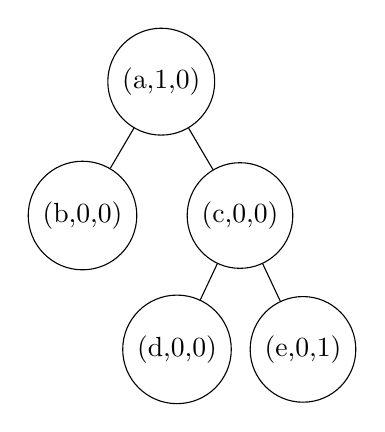
\begin{tikzpicture}[level distance=1.7cm,
				every node/.style={draw, circle, minimum size=5mm},
				level 1/.style={sibling distance=2cm},
				level 2/.style={sibling distance=1.6cm}]
			\node {(a,1,0)}
			child { node {(b,0,0)}}
			child { node {(c,0,0)}
					child {node {(d,0,0)}}
					child {node {(e,0,1)}} };
		\end{tikzpicture}
	\]

\end{example}

\begin{definition}["annotated tree"]
	Given a set of "nodes" $X$ and a "tree" t, we define an ""annotated tree"" as the pair $(t, X)$. This pair
	corresponds to a new "tree", where each "label" of a "node" is a pair consisting of the original "label" and a bit indicating whether the "node" belongs to the set $X$.

	We will use the notation $\intro*\bit X n $, where $n$ is a "node" of the "tree", to denote the bit indicating whether $n$ belongs to the set $X$.
\end{definition}

\begin{example}
	Let $t$ be the "tree" $a(b,c(d,e))$, and let $X = \{\varepsilon,0,11\}$.
	Then $(t, X)$ corresponds to the "annotated tree" :
	\[
		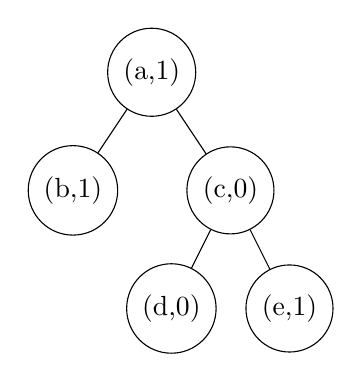
\begin{tikzpicture}[level distance=1.5cm,
				every node/.style={draw, circle, minimum size=5mm},
				level 1/.style={sibling distance=2cm},
				level 2/.style={sibling distance=1.5cm}]
			\node {(a,1)}
			child { node {(b,1)}}
			child { node {(c,0)}
					child {node {(d,0)}}
					child {node {(e,1)}} };
		\end{tikzpicture}
	\]
\end{example}


In the following, the "transition map" of the next automaton will be defined using a \texttt{match} syntax, where \texttt{\_}
denotes a wildcard that matches any value. Matches are evaluated from top to bottom, meaning the first rule that applies will be used.


\begin{lemma}\label{lem:atomic-a}
	Let $a \in \Sigma$. Over the alphabet $\Sigma \times \{0,1\}$, the "order-insensitive automaton"
	\[
		A = \big(\Sigma \times \{0,1\}, \{\mathrm{Yes}, \mathrm{No}\}, \init, \deltaA, \{\mathrm{Yes}\} \big)
	\]
	defined as follows:
	\[
		\begin{minipage}[t]{0.45\linewidth}
			\textbf{Initial states:}
			\[
				\begin{array}{ll}
					\init(a,1) & \Rightarrow \mathrm{Yes} \\
					\init(\_)  & \Rightarrow \mathrm{No}
				\end{array}
			\]
		\end{minipage}
		\hfill
		\begin{minipage}[t]{0.5\linewidth}
			\textbf{Transition map:}
			\[
				\begin{array}{ll}
					\deltaA(\_,\_,(a,1))                & \Rightarrow \mathrm{Yes} \\
					\deltaA(\mathrm{No},\mathrm{No},\_) & \Rightarrow \mathrm{No}  \\
					\deltaA(\_)                         & \Rightarrow \mathrm{Yes}
				\end{array}
			\]
		\end{minipage}
	\]
	decides the "atomic predicate" $a(x)$, where $x$ is a free first-order variable.
\end{lemma}

\begin{example}
	Let $t$ be the "tree" $a(b,c(d,e))$, and let $A$ be the automaton from \Cref{lem:atomic-a} for the letter $e$.
	Then the automaton $A$ will accept the "annotated tree" $(t, \{11\})$ as the "node" $11$ is labeled with $e$ in $t$. The "execution" of the automaton is illustrated in \Cref{fig:atomic-execution}.
\end{example}

\begin{figure}[h]
	\centering
	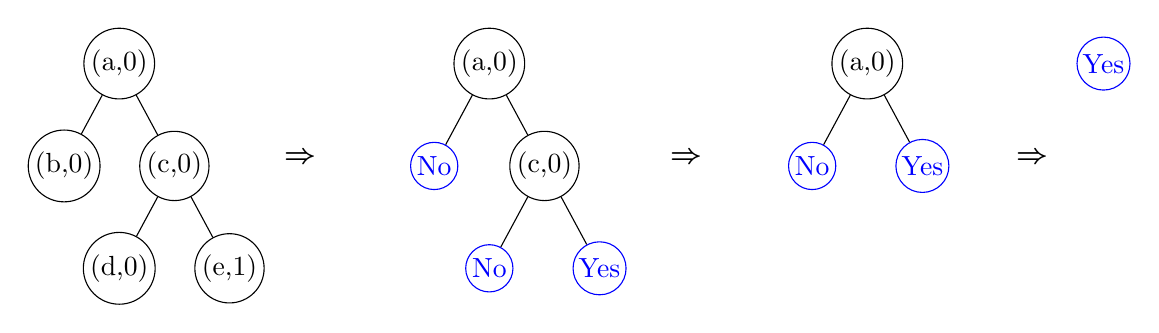
\begin{tikzpicture}[
			level distance=1.3cm,
			sibling distance=1.4cm,
			every node/.style={circle,draw,minimum size=6mm,inner sep=1pt},
			treenode/.style={circle,draw,minimum size=6mm,inner sep=1pt},
			scale=1, transform shape,
			state/.style={blue}
		]

		\node (t1) at (0,0) {(a,0)}
		child {node (t1b) {(b,0)}}
		child {node (t1c) {(c,0)}
				child {node (t1d) {(d,0)}}
				child {node (t1e) {(e,1)}}};

		\node at (2.3, -1.2) [draw=none] {$\boldsymbol{\Rightarrow}$};

		\node (t2) at (4.7,0) {(a,0)}
		child {node[state] (t2b) {No}}
		child {node (t2c) {(c,0)}
				child {node[state] (t2d) {No}}
				child {node[state] (t2e) {Yes}}};

		\node at (7.2, -1.2) [draw=none] {$\boldsymbol{\Rightarrow}$};

		\node (t3) at (9.5,0) {(a,0)}
		child {node[state] (t3b) {No}}
		child {node[state] (t3c) {Yes}};

		\node at (11.6, -1.2) [draw=none] {$\boldsymbol{\Rightarrow}$};

		\node[state] (t4) at (12.5,0) {Yes};

	\end{tikzpicture}
	\caption{"Execution" of the automaton from \Cref{lem:atomic-a} on the "annotated tree" $(a(b,c(d,e)), \{11\})$ for the label $e$.}
	\label{fig:atomic-execution}
\end{figure}

\begin{lemma}\label{lem:atomic-ancestor}
	Over the alphabet $\Sigma \times \{0,1\}^2$, the "order-insensitive automaton"
	\[
		A = \big(\Sigma \times \{0,1\}^2, \{\mathrm{Yes}, \mathrm{No}, \mathrm{FoundY}\}, \init, \deltaA, \{\mathrm{Yes}\} \big)
	\]
	defined as follows:
	\[
		\begin{minipage}[t]{0.45\linewidth}
			\textbf{Initial states:}
			\[
				\begin{array}{ll}
					\init(\_,\_,1) & \Rightarrow \mathrm{FoundY} \\
					\init(\_)      & \Rightarrow \mathrm{No}
				\end{array}
			\]
			\vfill
		\end{minipage}
		\hfill
		\begin{minipage}[t]{0.5\linewidth}
			\textbf{Transition map:}
			\[
				\begin{array}{ll}
					\deltaA(\mathrm{Yes}, \_, \_)           & \Rightarrow \mathrm{Yes}    \\
					\deltaA(\_, \mathrm{Yes}, \_)           & \Rightarrow \mathrm{Yes}    \\
					\deltaA (\mathrm{FoundY}, \_, (\_,1,0)) & \Rightarrow \mathrm{Yes}    \\
					\deltaA(\_, \mathrm{FoundY}, (\_,1,0))  & \Rightarrow \mathrm{Yes}    \\
					\deltaA(\mathrm{FoundY}, \_, (\_,0,0))  & \Rightarrow \mathrm{FoundY} \\
					\deltaA(\_, \mathrm{FoundY}, (\_,0,0))  & \Rightarrow \mathrm{FoundY} \\
					\deltaA(\_, \_, (\_,0,1))               & \Rightarrow \mathrm{FoundY} \\
					\deltaA(\_)                             & \Rightarrow \mathrm{No}
				\end{array}
			\]
		\end{minipage}
	\]
	decides the "atomic predicate" $x \ancestor y$, where $x$ and $y$ are free first-order variables.
\end{lemma}

\begin{example}
	Let $t$ be the "tree" $a(b,c(d,e))$, and let $A$ be the automaton from \Cref{lem:atomic-ancestor} for the "atomic predicate" $x \ancestor y$,
	where $x$ is the "node" labeled $c$ at position $1$ and $y$ is the "node" labeled $d$ at position $10$.
	The "execution" of the automaton is illustrated in \Cref{fig:atomic-execution-ancestor}.
\end{example}

\begin{figure}[h]
	\centering
	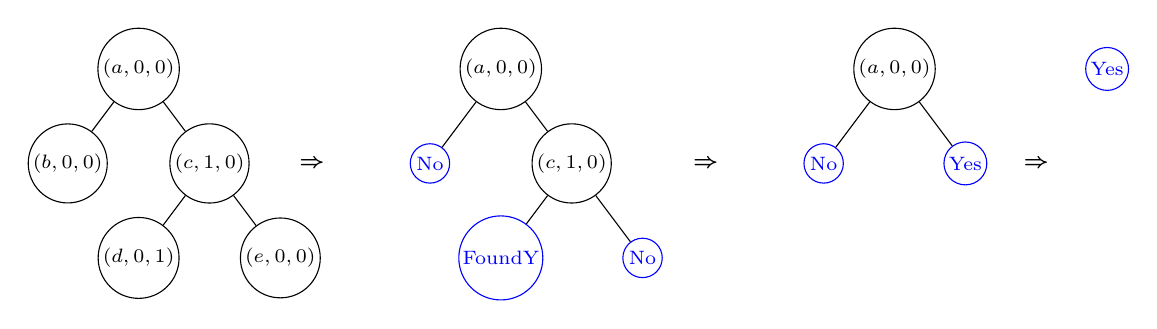
\begin{tikzpicture}[
			level distance=1.2cm,
			sibling distance=1.8cm,
			every node/.style={draw, circle, minimum size=5mm, inner sep=1pt, font=\scriptsize},
			state/.style={blue}
		]

		\node (t1) at (0,0) {$(a,0,0)$}
		child { node {$(b,0,0)$} }
		child { node {$(c,1,0)$}
				child { node {$(d,0,1)$} }
				child { node {$(e,0,0)$} }
			};

		\node at (2.2, -1.2) [draw=none] {$\boldsymbol{\Rightarrow}$};

		\node (t2) at (4.6,0) {$(a,0,0)$}
		child { node[state] {No} }
		child { node {$(c,1,0)$}
				child { node[state] {FoundY} }
				child { node[state] {No} }
			};

		\node at (7.2, -1.2) [draw=none] {$\boldsymbol{\Rightarrow}$}; 

		\node (t3) at (9.6,0) {$(a,0,0)$}
		child { node[state] {No} }
		child { node[state] {Yes} };

		\node at (11.4, -1.2) [draw=none] {$\boldsymbol{\Rightarrow}$};

		\node[state] at (12.3,0) {Yes};

	\end{tikzpicture}
	\caption{Execution of the automaton from \Cref{lem:atomic-ancestor} on the "annotated tree" $(a(b,c(d,e)),\{1\}, \{10\})$ for the nodes corresponding to the label $c$ and $e$.}
	\label{fig:atomic-execution-ancestor}
\end{figure}

We now have all of the ingredients to construct an "order-insensitive" "NBUA" for any "MSO-formula".

\begin{lemma}[from MSO to automata]\label{lem:MSO-to-aut}
	Let $\phi$ be an "MSO-formula". Then there exists an "order-insensitive" "NBUA" $A$ such that for every $t \in \tree_\Sigma$, we have:
	\[
		t \models \phi \quad \text{if and only if} \quad t \in \lang{A}.
	\]
\end{lemma}

\begin{proof}
	The construction proceeds by structural induction on $\phi$.

	"Atomic formulas" such as $a(x)$ and $x \ancestor y$ are handled directly by the automata
	in \Cref{lem:atomic-a,lem:atomic-ancestor}, which operate over "annotated trees" with the appropriate bit vectors.

	For conjunction and disjunction, we apply the induction hypothesis to obtain automata
	for the subformulas, then use the constructions from \Cref{lem:intersection,lem:union} to obtain an automaton for the whole expression.

	If $\phi = \lnot \psi$, then by the induction hypothesis we obtain an automaton for $\psi$. We apply
	\Cref{lem:complement} to obtain an automaton for $\phi$.

	Assume $\phi = \exists X.\psi(X)$, where $\psi$ has $n$ free variables and $X$ is the $n$-th one.

	By the induction hypothesis, we have an "order-insensitive" "DBUA" (since avery "NBUA" can be converted to a "DBUA")
	$A = (\Sigma \times \{0,1\}^n, Q, \init, \deltaA, F)$ that accepts the "language" of $\psi(X)$.

	We now construct an automaton that operates over $\Sigma \times \{0,1\}^{n-1}$, where $X$ is no longer explicitly assigned.
	Instead, we simulate all possible "annotations" for $X$, and "accept" if at least one such "annotation" makes $\psi(X)$ true.

	Define the new automaton $A' = (\Sigma \times \{0,1\}^{n-1}, \parts Q, \init', \deltaA', F')$ where:
	\begin{itemize}
		\item Initial states:
		      \[
			      \init'(a, \vec{b}) = \setdef{ \init(a, \vec{b}, b')} {b' \in \{0,1\} }
		      \]
		      That is, we simulate both possibilities for the missing bit.
		\item "Transition map":
		      \[
			      \deltaA'(P, Q, (a, \vec{b})) = \setdef{ \deltaA(p, q, (a, \vec{b}, b'))} {p \in P,\ q \in Q,\ b' \in \{0,1\} }
		      \]
		      Again, for every "node" guess if this it belongs to $X$, we compute the next "state" as if that guess were part of the input.
		\item "Accepting states":
		      \[
			      F' = \setdef{ P \subseteq Q} {P \cap F \neq \emptyset }
		      \]
		      The automaton accepts if one of the runs under some assignment for $X$ ends in an "accepting state".
	\end{itemize}

	This automaton simulates all possible choices of a "node" for $X$, \ie all possible  bit "annotations" for the $X$-variable.
	Since $A$ is "order-insensitive", and the construction treats all "nodes" symmetrically, $A'$ is also "order-insensitive".

	For $\phi = \exists x.\psi(x)$, we have that it's a particular case of the previous construction.

	Each inductive case preserves "order-insensitivity", and constructs an "NBUA" for the given formula. Thus, by induction on the structure of $\phi$,
	we obtain the desired automaton.
\end{proof}


\section{Uniformisation}\label{sec:uniformisation}
In this section we introduce the main concept of this work, "uniformisation" and we state and prove the main theorem, \Cref{thm:uniformisability-decision}.
\Cref{section:uniformisation-definitions} introduces the definitions and the main theorem, \Cref{section:uniformiser-automaton} defines the "uniformiser automaton",
and \Cref{section:correctness} and \Cref{section:soundness} prove the correctness and soundness of the algorithm, respectively.

\subsection{Definitions and statement of the main theorem}\label{section:uniformisation-definitions}

We begin by formalising the core concepts.

\begin{definition}\label{def:uniformiser}
	\AP An "MSO-formula" $\psi(X)$ is a ""uniformiser"" of an "MSO-formula" $\phi(X)$ if, for all "trees" $t$, the following hold:
	\begin{enumerate}
		\item There exists at most one set $X$ such that $t \models \psi(X)$.
		\item If there exists a set $X$ such that $t \models \phi(X)$, then there exists a set $Y$ such that $t \models \psi(Y) \land \phi(Y)$.
	\end{enumerate}
	\AP An "MSO-formula" $\phi(X)$ is said to be ""uniformisable"" if it admits a "uniformiser".
\end{definition}

\begin{remark}\label{remark:uniformisability}
	An equivalent way to express that $\phi(X)$ is "uniformisable" is that there exists an "MSO-formula" $\psi(x)$ such that, for all "trees" $t$:
	\[
		t \models \exists X.\, \phi(X) \quad \text{implies} \quad t \models \phi(\setdef{x}{t \models \psi(x)}).
	\]
	Note that here we use a set defined by comprehension, which is not in the syntax of plain "MSO logic".
	This is for commodity and can be easily translated into a syntactically correct equivalent statement.
\end{remark}

We can now state the main result of this work.
\begin{theorem} \label{thm:uniformisability-decision}\label{theorem:main}
	There exists an algorithm which, given an "MSO-formula" as input, decides whether it has a "uniformiser" over "finite unordered binary trees".
\end{theorem}

In fact, it is a consequence of a more precise result, \Cref{lemma:main}, that we state now, though all the definitions necessary have not yet been provided.
\begin{lemma}\label{lem:main-result}\label{lemma:main}
	For all "MSO-formulas" $\phi(X)$, the following statements are equivalent:
	\begin{enumerate}
		\item $\phi(X)$ is "uniformisable". \label{lem:main-result-1}
		\item For all "trees" $t$ that models $\phi(X)$ for some~$X$, $t$ models~$\phi(X)$ for some "definable"~$X$. \label{lem:main-result-2}
		\item For all "trees" $t$ that models $\phi(X)$ for some~$X$, $t$ models~$\phi(X)$ for some~$X$ invariant under the automorphisms of~$t$ (\ie such that $\sigma(X) = X$ for all $\sigma \in \Aut(t)$). \label{lem:main-result-3}
		\item The "uniformiser automaton" of~$\phi(X)$ is "universal". \label{lem:main-result-4}
	\end{enumerate}
	As as consequence, "uniformisability@uniformisable" of "MSO" over trees is decidable.
\end{lemma}

In the rest of this section, we recall the definitions of "definable" sets and invariance under "automorphisms" from which we immediately get the implications from
\Cref{lem:main-result-1} to \Cref{lem:main-result-2}, and from \Cref{lem:main-result-2} to \Cref{lem:main-result-3}. The "uniformiser automaton"
is then defined in the next section, \kCref{uniformiser automaton}. The implication from \Cref{lem:main-result-3} to \Cref{lem:main-result-4} is then the subject of
\Cref{lemma:not-universal-implies-non-invariant} in \Cref{section:soundness} and the implication from~\Cref{lem:main-result-4} to \Cref{lem:main-result-1} is stated in
\Cref{lemma:universal-implies-uniformisable}, \Cref{section:correctness}.

\begin{definition}["definable set"]\label{def:definable}
	\AP Let $t$ be a "tree". A set $X \subseteq \Nodes t$ is ""definable"" if there exists an
	"MSO-formula" $\phi(x)$ such that $X = \setdef{x}{t \models \phi(x)}$.
\end{definition}

In particular, if $\phi(X)$ is "uniformisable", there exists a "uniformiser" $\psi(x)$ such that for all "trees" $t$,
we have that the set $X_d = \setdef{x}{t \models \psi(x)}$ is "definable" in $t$ and models $\phi(X_d)$ if $t$ models $\exists X.\, \phi(X)$,
see \Cref{remark:uniformisability}.
This proves the implication from \Cref{lem:main-result-1} to \Cref{lem:main-result-2} in \Cref{lemma:main}.

Another concept used in this section is the one of "automorphisms" of "trees".
\begin{definition}["automorphism"]\label{def:automorphism}
	\AP An ""automorphism"" of a "tree" $t$ is a bijection $\sigma : \Nodes t \to \Nodes t$ preserving the tree structure:
	if $u$ is a "child" of $v$, then $\sigma(u)$ is a "child" of $\sigma(v)$, and $\sigma$ preserves the labels of nodes.
	The group of all automorphisms of $t$ is denoted $\intro* \Aut(t)$.
\end{definition}

In other words, an "automorphism" is a symmetry of the "tree" that rearranges its nodes while preserving the ancestor relation and labels.
Let us illustrate this concept with an example.


\begin{example}
	We compare the automorphism groups of two binary trees.

	\begin{center}
		\begin{tabular}{cc}
			% First tree
			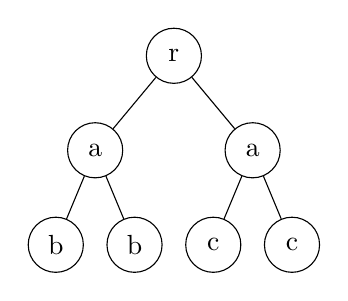
\begin{tikzpicture}[level distance=1.2cm,
					every node/.style={draw, circle, minimum size=7mm},
					level 1/.style={sibling distance=2cm},
					level 2/.style={sibling distance=1cm}]
				\node {r}
				child { node {a}
						child {node {b}}
						child {node {b}} }
				child { node {a}
						child {node {c}}
						child {node {c}} };
			\end{tikzpicture}
			                           &
			% Second tree
			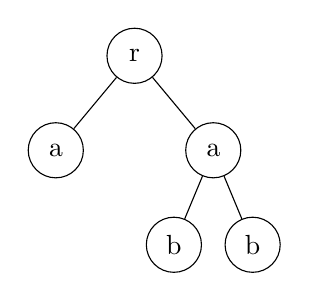
\begin{tikzpicture}[level distance=1.2cm,
					every node/.style={draw, circle, minimum size=7mm},
					level 1/.style={sibling distance=2cm},
					level 2/.style={sibling distance=1cm}]
				\node {r}
				child { node {a} }
				child { node {a}
						child {node {b}}
						child {node {b}} };
			\end{tikzpicture}
			\\
			\textbf{Tree A: Symmetric} & \textbf{Tree B: Asymmetric}
		\end{tabular}
	\end{center}

	\textbf{Tree A} is a complete "binary tree" of height 2. In this case, there are 8 "automorphisms", corresponding to all possible ways of swapping left and right "children" at each level.

	\textbf{Tree B}, on the other hand, is asymmetric. The left "child" of the root is a "leaf", while the right "child" is an "internal node" with two "children".
	Since these "subtrees" are not structurally the same, the only "automorphisms" are:
	\begin{itemize}
		\item the identity (doing nothing), and
		\item swapping the two "children" of the right "subtree".
	\end{itemize}
\end{example}


The next lemma states an intuitive property of "definable" sets in relation to "automorphisms", we propose an intuitive proof idea.

\begin{lemma}\label{lem:def-aut}
	If $X$ is "definable" in a "tree" $t$, then $\sigma(X) = X$ for all $\sigma \in \Aut(t)$ .
\end{lemma}

\begin{proof}[Idea of a proof]
	If $X$ is "definable", there exists an "MSO-formula" $\phi(x)$ such that $X = \setdef{x}{t \models \phi(x)}$.
	We want to show that for all $\sigma \in \Aut(t)$ and all $x \in X$, we have $t \models \phi(\sigma(x))$.
	Since $\sigma$ is a bijection, this suffices to conclude $\sigma(X) = X$.

	The idea is that an "MSO-formula", by construction, cannot distinguish between "nodes" that are mapped to each other by "automorphisms", since
	the only relationship between "nodes" that an "MSO-formula" can express is the "ancestor relation", which is preserved by "automorphisms".

	The proof proceeds by induction on the structure of $\phi$. "Atomic formulas" are invariant under "automorphisms" by definition,
	since "automorphisms" preserve the tree structure and labeling. The logical connectives (conjunction, disjunction, negation)
	and quantifiers preserve this invariance, so the property holds inductively.

	Therefore, for all $x \in X$, we have $t \models \phi(x)$ implies $t \models \phi(\sigma(x))$, and hence $\sigma(x) \in X$. Thus, $\sigma(X) = X$.
\end{proof}

The implication from \Cref{lem:main-result-2} to \Cref{lem:main-result-3} in \Cref{lemma:main} is a direct consequence of \Cref{lem:def-aut}.

\subsection{The uniformiser automaton}\label{section:uniformiser-automaton}
Let us fix an "MSO-formula" $\phi(X)$. At very high level, what we aim at is a procedure that would solve a statement of the form\footnote{This is an intuition, and not a valid formula of MSO.}:
\[
	(\exists X.\, \phi(X)) \rightarrow (\exists X.\, \phi(X) \text{ and $X$ is invariant under "automorphism"}).
\]
We aim to build an automaton that somehow accepts the "trees" for which this property holds.
This is the "uniformiser automaton" for the formula, that we describe below. We then show in \Cref{lemma:universal-implies-uniformisable} that if it is "universal",
then $\phi(X)$ is "uniformisable", and in \Cref{lemma:not-universal-implies-non-invariant} that if it is not "universal", then there exists a
"tree"~$t$ that models~$\phi(X)$ for some~$X$, but does not model~$\phi(X)$ for some~$X$ that would be invariant under the "automorphisms" of~$t$.
\begin{definition}["uniformiser automaton"]
	\AP Let $\phi(X)$ be an "MSO-formula" and $A = (\Sigma \times \{0,1\}, Q, \init, \deltaA, F)$ its "DBUA". The ""uniformiser automaton"" is defined as
	\[
		\intro* \Ua = (\Sigma, \parts{Q} \times \parts{Q}, \init_U, \deltau, F')
	\]
	where:
	\begin{itemize}
		\item $\init_U(a) = (\init(a,"*"), \init(a,"*"))$
		      \itemAP $\intro*\deltau((X,X'),(Y,Y'),a) = (\deltaA(X,Y,(a,*)), \deltauu(X',Y',a))$ with:
		      \[
			      \intro*\deltauu(X',Y',a) = \begin{cases}
                      \setdef{\deltaA(p,p,(a,b))}{p \in X', b \in \set{0,1}} & \text{if } X = Y \text{ and } X' = Y'  \\
				      \deltaA(X',Y',(a,"*"))                                 & \text{otherwise}
			      \end{cases}
		      \]
		\item $F' = \setdef{(X,X')}{(X \cap F \neq \emptyset) \Rightarrow (X' \cap F \neq \emptyset)}$
	\end{itemize}
	\AP Using the notation $\deltaA(X,Y,(a,""*""))$ for $\bigcup_{b \in \set{0,1}} \deltaA(X,Y,(a,b))$, and $\init(a,\reintro{*})$ for $\bigcup_{b \in \set{0,1}} \init(a,b)$.
	Note that in this definition, the automaton $A$ corresponds to the automaton for the "formula" $\phi(X)$, particular if $A$ "accepts" a "tree" $t$ then
	there exists a set $X$ such that $t \models \phi(X)$.
\end{definition}


Intuitively, $\Ua$ checks whether $\phi(X)$ has a witness, and attempts to reconstruct a witness invariant under "automorphisms" using symmetry constraints.

Each "state" of the "uniformiser automaton" is a pair of "states" of the original automaton for $\exists X.\phi(X)$.
The first component represents a standard "run" of said automaton (checking if the formula $\phi(X)$
can be modeled), while the second component simulates a restricted "run" that captures a solution that is invariant under "automorphisms".
When both sides behave identically on a given "subtree", that is, when the shape and labels of the "tree" do not allow
us to distinguish between them, the automaton enforces that they must transition identically, ensuring symmetry. This restriction
is what guarantees that the selected set $X$ is invariant under "automorphisms".

\begin{definition}["uniformisability checking algorithm"]
	\AP Given an "MSO-formula" $\phi(X)$ as an input, the ""uniformisability checking algorithm"" constructs the "uniformiser automaton" for $\phi(X)$
	and checks whether it is "universal", using the algorithm from \Cref{coro:univeral-Reach}. If it is "universal", then the algorithm returns 'yes', indicating
	that $\phi(X)$ is "uniformisable". Otherwise, it returns 'no', indicating that $\phi(X)$ is not "uniformisable".
\end{definition}

In the rest of this section, we will prove that this algorithm is correct and sound, leading to the main result of this article, \Cref{thm:uniformisability-decision}.

\subsection{Correctness}\label{section:correctness}

In this section, we prove the correctness of the "uniformisability checking algorithm", which is the
implication from \Cref{lem:main-result-4} to  \Cref{lem:main-result-1} in \Cref{lemma:main}.
This is what states the next lemma.

\begin{lemma}\label{lemma:universal-implies-uniformisable}
	Let $\phi(X)$ be an "MSO-formula", if the "uniformiser automaton" of $\phi(X)$ is "universal" then $\phi(X)$ is "uniformisable".
\end{lemma}

\begin{proof}
	Let $A =  (\Sigma \times \{0,1\}, Q, \init, \deltaA, F)$ be the automaton for $\phi(X)$ and lets suppose that
	$\Ua = (\Sigma, \parts Q \times \parts Q,\init', \deltaA', F')$ the "uniformiser automaton" of $\phi(X)$ is "universal".
	We need to exhibit a "uniformiser" for $\phi(X)$.

	\AP We start by introducing a set of choice functions, their purpose is that, given a set of "states" of $A$, they will choose
	a particular "state" of $A$ following some restrictions. This means that we will have a way to reconstruct a "run" of $A$ over a "tree" $t$ "annotated" with a
	particular set $X$ of "nodes" of $t$, that satisfies the restrictions of $\deltauu$, and that is unique.
	\begin{itemize}
		\itemAP We first introduce $\intro*\choiceN : \parts Q \times \parts Q \times Q \times \Sigma \to Q \times Q \times \set{0,1}$
		that given $(X',Y',r,a)$ chooses a triple $(b,p,q)$ such that, if $r \in \deltauu(X',Y', a)$ then $\deltaA(p,q,(a,b)) = r$ where $p \in X', q \in Y'$
		and if $X = Y$ and  $X' = Y'$ then $p = q$. This function will select the next "state" when we are at an "internal node" of the "tree".
		\itemAP We also introduce $\intro* \choiceL : Q \times \Sigma \to \set{0,1} $, which chooses $b$ such that $p = \init((a,b))$. This function
		will select the next "state" when we are at a "leaf" of the "tree".
		\itemAP
		Finally, we need to choose from a "final state": $\intro* \choiceF : \parts Q \to  Q$ where
		$\choiceF (X) = q$ such that if $X \cap F \neq \emptyset$ then $q \in X \cap F$. This will correspond to the "final state" of our "run".
	\end{itemize}
	If the premises are not satisfied in any of the cases, then these choice functions return an arbitrary value. Since th number of "states" is finite, such choice 
    functions exist for an arbitrary ordering of the "states" of $A$.

	Now, thanks to the choice function, we can define a function $\rhou : \Nodes t \to Q$ that corresponds to a "run" $A$ over $t$ "annotated" with a set $\Xu$ of "nodes" defined later.
	The fact that it is a "run" will be proved later.

	\AP We define the set $\intro*\Xu$ and the  $\intro*\rhou$  by induction on the depth of the "node" as follows:
	\begin{itemize}
		\item For the "root", we define $\rhou(\varepsilon) = \choiceF(\deltauu(t))$.
		\item For all "internal nodes" $x$ with "children" $y$ and $z$.

		      Let $(p,q,v) = \choiceN(\deltauu(\subtree t y), \deltauu(\subtree t z), \rhou(x), \tlabel t x)$, we define $\rhou(y)=p$, $\rhou(z)=q$, and $x \in \Xu$ if and only if $b = 1$.
		\item For all "leaves" $x$, let $b$ be ~$b = \choiceL(p, \tlabel t x)$ we define $\rhou (x) = p$, where $x \in \Xu$ if and only if $b = 1$.
	\end{itemize}

	\begin{claim}
		We claim now that the $\rhou$ is well defined, unique, and indeed a "run" of $A$ over $(t,\Xu)$.
	\end{claim}

	\begin{proof}[Proof of the claim]
		The proof proceeds by top-down induction.
		\begin{itemize}
			\item For $\varepsilon$, the "root" of $t$, we have that $\rhou(\varepsilon) = \choiceF(\deltauu(t))$, since $\choiceF$ is deterministic, $\rhou(\varepsilon)$ is unique.
			\item For the "internal nodes" $x$ with "children" $y$ and $z$, there exists $r \in Q$, such that $\rhou (x) = r$ by the induction hypothesis. Then,
			      since $\choiceN$ is deterministic, there exists a unique tuple $(p,q,b)$ such that $(p,q,b) = \choiceN(\deltauu(\subtree t y), \deltauu(\subtree t z), r, \tlabel t x)$.
			      We have that $\rhou(y) = p$ and $\rhou(z) = q$, which verify that $\deltaA(p,q,(\tlabel t x,b)) = r$. We also have that $x \in \Xu$ if and only if $b = 1$.
			      This is then a valid "run" of $A$ over $(t,\Xu)$
			\item For a "leaf" $x$ of "label" $a$, by the induction hypothesis we have that $b = \choiceL(a, \rhou(x))$ which is well defined since $a \in \Sigma$ and unique.
			      We also have that $x \in \Xu$ if and only if $b = 1$ and $\rho(x) = \init((a,b))$.
		\end{itemize}
		The claim is proved.
	\end{proof}

	In particular, it is a "run" that satisfies the restrictions of $\deltauu$ and so if $\rhou(x) \in F$ then $\Xu$ models $\phi(X)$.

	\AP We are now ready to define an "MSO-formula" $\intro*\unif (X)$ that witnesses that $\phi(X)$ is "uniformisable".
	This formula simply states using the MSO-syntax the existence of the "run" $\rhou$ described above, \ie
	$t \models \unif(X)$ if and only if $X=\Xu$.

	\AP Given a set of "states" $P$, from \Cref{thm:MSO-NBUA} there exists a formula $\intro* \ustate_P(x)$ such that
	$t \models \ustate_P(x)$ if and only if  $\deltauu(\subtree t x) = P$.

	Let $k = \abs Q$, we will define 5 subformulas of $\unif(X)$.

	\begin{eqnarray*}
		\AP \intro* \singleState (X_{p_1}, \ldots, X_{p_k})  &=& \forall x, \bigvee_{1 \leq i \leq k} X_{p_i} (x)\\
		&\land& \forall x, \bigwedge_{1 \leq i, j \leq k, i \neq j} \lnot(X_{p_i} (x) \land X_{p_j}(x))
	\end{eqnarray*}
	This "MSO-formula" states that every node is assigned to exactly one of the $X_{p_i}$, which are the "states" of the automaton $A$.

	\begin{equation*}
		\AP \intro*	\rootNode (X_{p_1}, \ldots, X_{p_k})  = \forall x, \treeroot(x) \ra (\bigvee_{p_i \in \choose \deltauu(\varepsilon)} X_{p_i}(x))
	\end{equation*}
	We now state that the "root" of the "tree" is assigned to the state chosen by $\choiceF$.

	\begin{equation*}
		\AP \intro* \inSet_b (X, x)  = (b = 1) \Leftrightarrow X(x)
	\end{equation*}
	This formula can be expressed in real MSO syntax, but we propose a more intuitive definition.

	\begin{equation*}
		\AP \intro* \leafNode (X_{p_1}, \ldots, X_{p_k})  = \forall x \left( \leaf(x) \rightarrow \bigvee_{\substack{(a, q) \in \init,\\ \choiceL(a,q) = b}} X_i(x) \land  \inSet_b (X,x)  \right)
	\end{equation*}

	This "MSO-formula" verifies that the "state" of a "leaf" is the one chosen by $\choiceL$, and that the "leaf" is in the set $X$ if and only if $b = 1$.

	\begin{eqnarray*}
		\AP \intro* \innerNodes (X_{p_1}, \ldots, X_{p_k}, X)  &=& \forall x \forall y \forall z, \children (x,y,z) \ra \\
		&& \bigvee_{ \substack{(P',Q',a,R')\in \deltauu, \, r \in R', \\ \choiceN(P',Q',a,r) = (p,q,b)}} \Big( \ustate_{P'}(x) \land \ustate_{Q'}(y) \\
		&& \qquad \land \  X_p(x) \land X_q(y) \land a(z) \land X_r(z) \land  \inSet_b(X,x)\Big)
	\end{eqnarray*}
	That last formula states that for every "internal node" $x$ with "children" $y$ and $z$, the "state" of $x$ is the one chosen by $\choiceN$,
	that the "states" of $y$ and $z$ are the ones chosen by $\choiceN$, and that "node" is in the set $X$ if and only if $b = 1$.


	We can now define $\unif(X)$:
	\begin{eqnarray*}
		\unif (X) &=& \exists X_{p_1}, \ldots, \exists X_{p_k}, \singleState (X_{p_1}, \ldots, X_{p_k}) \\
		&\land& \leafNode (X_{p_1}, \ldots, X_{p_k})\\
		&\land& \rootNode (X_{p_1}, \ldots, X_{p_k})\\
		&\land& \innerNodes (X_{p_1}, \ldots, X_{p_k}, X)
	\end{eqnarray*}
	$\unif(X)$ describes the run $\rhou$ over $(t,\Xu)$ and has a unique solution, $\Xu$.

	Lets show that $\unif(X)$ is a "uniformiser" for $\phi(X)$.
	Since $\Ua$ is "universal" the we have that, whenever $\phi(X)$ has a solution for a "tree" $t$, then there exists an "accepting run" $\rho$ of $\Ua$ over $t$
	such that $\rho(\varepsilon) = (X,X')$ and such that $X \cap F \neq \emptyset$. Since the "run" is "accepting" $X' \cap F \neq \emptyset$, and we have that
	$\rhou$ is then well defined and $\unif(X)$ has a solution. Since $\rhou$ is a run of $A$, then we have that $\Xu$ is also a solution of $\phi(X)$, an since
	$\unif(X)$ as a unique solution, we have that $\unif(X)$ is indeed a "uniformiser" for $\phi(X)$.

\end{proof}

\subsection{Soundness}\label{section:soundness}

In this section, we prove the soundness of the "uniformisability checking algorithm", by compleating the proof of \Cref{lem:main-result-3} to
\Cref{lem:main-result-4} in \Cref{lemma:main} by contraposition.
This chain of implications states that if $\phi(X)$ is "uniformisable", then the "uniformiser automaton" of $\phi(X)$ is "universal", \ie that the algorithm is sound.

\begin{lemma}\label{lemma:not-universal-implies-non-invariant}
	Let $\phi(X)$ be an "MSO-formula", if the "uniformiser automaton" of $\phi(X)$ is not  "universal",
	then there exists a "tree"~$t$ that models~$\phi(X)$ for some~$X$, but does not model~$\phi(X)$ for some~$X$
	that would be invariant under the automorphisms of~$t$.
\end{lemma}

\begin{proof}
	Let $A =  (\Sigma \times \{0,1\}, Q, \init, \deltaA, F)$ be the automaton for $\phi(X)$ and lets suppose that
	$\Ua = (\Sigma, \parts Q \times \parts Q,\init', \deltaA', F')$ the "uniformiser automaton" of $\phi(X)$ is not "universal".
	We will show that there exists a "tree" $t$ that models  $\phi(X)$ for some $X$, but does not model $\phi(X)$ for
	some $X$ that is invariant under the "automorphisms" of $t$.

	Since $\Ua$ is not "universal", there exists $(R,R') \in \Reach \Ua$, such that $R \cap F \neq \emptyset$ and $R' \cap F = \emptyset$.
	We want to define a "tree" $t_{R,R'}$ such that
	\begin{enumerate}
		\item $R \subseteq \{ \deltaA_A (t_{R,R'},X) \mid X \subseteq \Nodes {t_{R,R'}}\}$ \label{lem:prop1}
		\item $\{ \deltaA_A (t_{R,R'},X) \mid \forall \sigma \in \Aut(t_{R,R'}), \sigma(X) = X\} \subseteq R'$\label{lem:prop2}
		\item $\interpret \Ua {t_{R,R'}} = (R,R')$\label{lem:prop3}
	\end{enumerate}

	We proceed by induction over the construction of elements in $\Reach {\Ua}$:

	If $(T,T') = (\init(a,"*"), \init (a, "*"))$ for $a \in \Sigma$, then \Cref{lem:prop1} and \Cref{lem:prop3} are trivially satisfied and we have that
	$\Aut (a) = \{\text{id}\}$, so \Cref{lem:prop2} is also satisfied.

	If $(T,T') = \deltaA_{\Ua}((P,P'),(Q,Q'),a)$ for $a \in \Sigma$ and $P,P',Q,Q' \in \Reach \Ua$, then by the induction hypothesis there exists
	$t_{P,P'}$ and $t_{Q,Q'}$ that verify the hypothesis. We can construct $t_{T,T'} = a(t_{P,P'},t_{Q,Q'})$. Lets prove that it satisfies the
	three properties.

	We will prove \Cref{lem:prop3}.
	By definition of $\interpret \Ua {\cdot}$,
	$\interpret \Ua {t_{T,T'}} = \deltaA_{\Ua} (\interpret \Ua {t_{P,P'}}, \interpret \Ua {t_{Q,Q'}}, a)$.
	If we use \Cref{lem:prop3} of the induction hypothesis we deduce that
	$\deltaA_{\Ua} (\interpret \Ua {t_{P,P'}}, \interpret \Ua {t_{Q,Q'}}, a) = \deltaA_{\Ua} ((P,P'), (Q,Q'), a)$
	And by definition of $(T,T')$, $\deltaA_{\Ua} ((P,P'), (Q,Q'), a) = (T,T')$.
	\Cref{lem:prop3} is then verified.

	By definition, $T = \deltaA_A(P,Q,(a,"*"))$. Since by \Cref{lem:prop1} of the induction hypothesis $P \subseteq \{ \deltaA_A (t_{P,P'},X) \mid X \subseteq \Nodes {t_{P,P'}}\}$
	and $Q \subseteq \{ \deltaA_A (t_{Q,Q'},X) \mid X \subseteq \Nodes {t_{Q,Q'}}\}$  we have that
	$T = \deltaA_A(P,Q,(a,"*")) \subseteq \{ \deltaA_A (t_{T,T'},X) \mid X \subseteq \Nodes {t_{T,T'}}\}$. We have proven \Cref{lem:prop1}.

	We will prove \Cref{lem:prop2} by case distinction.
	Let $X \subseteq \Nodes {t_{P,P'}}$ such that $\forall \sigma \in \Aut (t_{T,T'}), \sigma(X) = X$, we introduce the
	sets $X_1 = X \cap \Nodes {t_{P,P'}}$ and $X_2 = X \cap \Nodes {t_{Q,Q'}}$.
	\begin{itemize}
		\item Lets suppose $t_{P,P'} \cong t_{Q,Q'}$.
		      By \Cref{lem:prop3} of the induction hypothesis
		      $\interpret \Ua {t_{P,P'}} = (P,P')$ and $\interpret \Ua {t_{Q,Q'}} = (Q,Q')$, since $\interpret \Ua {\cdot}$ is a function
		      and $\interpret \Ua {t_{P,P'}} = \interpret \Ua {t_{Q,Q'}}$, we have that $P = Q$ and $P' = Q'$.

		      Let $\sigma$ be the "automorphism" over $\Nodes{T,T'}$ that swaps  $t_{P,P'}$ and $t_{Q,Q'}$.
		      We have that $\sigma (X) = X$. Since $\deltaA(X) = X$, $\deltaA$ must map $X_1$ to $X_2$, and the same is true for
		      $X_2$. So we have that $X_1 = X_2$ which means that $\sigma(X_1) = X_1$ and $\sigma(X_2) = X_2$. By construction we have that $p := \deltaA_A(t_{P,P'}, X_1) =  \deltaA_A(t_{Q,Q'}, X_2)$.
		      Using \Cref{lem:prop2} of the induction hypothesis, we find that $p \in P'$. So
		      $\deltaA_A (t_{T,T'}, X) = \deltaA_A(p,p,(a, \bit X {\treeroot})) \in T'$.

		\item Lets suppose $t_{P,P'} \ncong t_{Q,Q'}$, in this case we have that $P' \neq Q'$ or $P \neq Q$ and thus $T' = \deltauu (P',Q',a) = \deltaA_a(P',Q',(a,"*"))$.

		      We have to prove that
		      $\{ \deltaA_A (t_{T,T'},X) \mid \forall \sigma \in \Aut(t_{T,T'}), \sigma(X) = X\} \subseteq T'$.
		      Let $\sigma \in \Aut(t_{T,T'})$. Since $t_{P,P'} \ncong t_{Q,Q'}$, $\sigma$ cannot swap $t_{P,P'}$ and
		      $t_{Q,Q'}$.
		      Since we have that $\sigma(X) = X$, then we deduce that $\sigma(X_1) = X_1$ and
		      $\sigma(X_2) = X_2$, because $\sigma$ must act on the "subtrees" independently (because the "subtrees" are not isomorphic).
		      Let $p := \deltaA_A (t_{P,P'}, X_1)$ and $q := \deltaA_A (t_{Q,Q'}, X_2)$.
		      Using \Cref{lem:prop2} of the induction hypothesis we deduce that $p \in P'$ and $q \in Q'$.
		      So $\deltaA_A (t_{T,T'}, X) = \deltaA_A(p,q,(a, X(\treeroot))) \in T'$.
	\end{itemize}
	We have proved the three properties.

	Lets prove the lemma by exhibiting that no $X$ verifying $t_{R,R'} \models \phi(X)$ is invariant under the "automorphisms" of $t_{R,R'}$.
	Since $R \cap F \neq \emptyset$, there exists $X$ that models $\phi(X)$ and  belonging to $R \cap F$. We can use \Cref{lem:prop1} to deduce that
	$X \in \{ \deltaA_A (t_{R,R'},X) \mid X \subseteq \Nodes {t_{R,R'}}\} \cap F$.
	We also know that $R' \cap F = \emptyset$, we can the deduce that $\{ \deltaA_A (t_{R,R'},X) \mid \forall \sigma \in \Aut(t_{R,R'}), \sigma(X) = X\} \cap F = \emptyset$
	thanks to \Cref{lem:prop2}. So we know that $X \notin \{ \deltaA_A (t_{R,R'},X) \mid \forall \sigma \in \Aut(t_{R,R'}), \sigma(X) = X\} \cap F = \emptyset$ which means that no
	$X$ satisfying $t_{P,P'} \models \phi(X)$ is invariant under the "automorphisms" of $t_{R,R'}$.
\end{proof}

\Cref{lem:main-result} is then proved. We can conclue with a simple proof of our main theorem.

\begin{proof}[Proof of \Cref{thm:uniformisability-decision}]
	\Cref{lem:main-result} states the equivalence between the "uniformisability" of a formula $\phi(X)$ and the "universality" of its "uniformiser automaton" $\Ua$.
	We can use the "uniformisability checking algorithm" to construct $\Ua$ and check whether it is "universal". This algorithm decides whether $\phi(X)$ is "uniformisable".
\end{proof}

\section{Conclusion}\label{sec:conclusion}

We proved that the uniformisation problem for MSO formulas over unordered finite binary trees is decidable, using automata theory based
on "order-insensitive bottom-up automata". The construction also gives a way to extract a "uniformiser" when one exists. Along the way,
we showed that "uniformisability" coincides with "definability" and "automorphism" invariance in this setting.

There are several interesting directions for future work. While the decidability of the general case for infinite trees is a hard open question,
it could be worth investigating whether this approach could help identify subclasses of infinite trees for which "uniformisability" is decidable.
Similarly, it would be natural to consider extending these results to unranked trees, where nodes can have an arbitrary number of children.

\bibliographystyle{plainurl}
\bibliography{tree-uniformisation}

\end{document}
